\chapter{Stationary phase}
The Laplace method gave us a way of evaluating the integral when the integrand was sharply peaked (dominant contribution was coming from the region underneath the peak). The stationary phase method is used when the integrand is \emph{rapidly oscillating}. Here the integral is dominated by the region where the rapid oscillations slow down (rapid oscillations cancel out in other regions).\\
\ \newline
\paragraph{Example 1:} Consider
\begin{align*}
	I(\omega) &= \int_{a}^{b} \cos \omega t \, \md t \\
	&= \frac{1}{\omega}(\sin \omega b - \sin \omega a ) \sim O\left(\frac{1}{\omega }\right)
\end{align*}
As $\omega \rightarrow \infty$, $I(\omega) \rightarrow 0$ because of lots of rapid cancellations. The amount that does not cancel is roughly related to the spacing -- time period $T$ -- which is $O(1/\omega)$.

\paragraph{Example 2:} Now consider a slowly varying amplitude modulation to the rapidly varying $\cos$ function
\begin{align*}
	I(\omega) &= \int_{a}^{b} f(t) \cos \omega t \, \md t \\
	&= \left| f(t) \frac{\sin \omega t}{\omega} \right|^b_a - \frac{1}{\omega }\int_{a}^{b} f'(t) \sin \omega t \, \md t \\
	& = O\left(\frac{1}{\omega}\right) + o\left(\frac{1}{\omega}\right)
\end{align*}
Again expect $I(\omega) = O(1/\omega)$ as $\omega \rightarrow \infty$ due to oscillatory cancellations. The second term decays faster by an extra $1/\omega$ factor due to a similar reasoning.


\paragraph{Example 3:} More generally, we can estimate
\begin{gather*}
	I(x) = \int_{a}^{b} f(t) \me^{\mi x \psi(t)} \qquad x \rightarrow \infty
\end{gather*} 
Start by trying integration by parts on the problem:
\begin{align*}
	I(x) &= \left.\frac{f}{\mi x \psi '} \me^{\mi x \psi} \right|^b_a - \frac{1}{\mi x} \int_{a}^{b} \me^{\mi x \psi } \left(\frac{f}{\psi'}\right)' \md t \\
	&= O\left(\frac{1}{x}\right) + o\left(\frac{1}{x}\right)
\end{align*}
Following caveats should be noted:
\begin{itemize}
	\item $f/\psi'$ should be smooth on $[a,b]$ 
	\item and $\neq 0$ at both $t=a$ and $t=b$ so that the first term may provide the dominant contribution
	\item and need $\psi$ to be continuously differentiable on $[a,b]$ and not constant on any subinterval 
\end{itemize}
{\bf NB} But what if $\psi'=0$ somewhere on $[a,b]$? That is the point of stationary phase and of most interest to us. $\psi(t)$ is often called the phase of $\me^{\mi x \psi}$ (really, $x\psi$ is the phase, but we do not make the distinction). The major contribution to $I(x)$ comes from neighbourhood of such points. Why? Because the ``oscillatory cancellations effect" weakens/disappears near points of stationary phase. To see this, expand $\psi(t)$ about some point $t_0$
\begin{align*}
	\me^{\mi x \psi(t)} = \me^{\mi x \left[\psi(t_0) + (t-t_0) \psi'(t_0) + \frac{1}{2}(t-t_0)^2 \psi''(t_0) + \dots\right]} 
\end{align*}
Note that $x\psi'(t_0)$ is the local oscillation frequency at $t_0$. $x \psi(t_0)$ is just a constant multiplicative factor. Can show that if $\psi'(c)=0$ but $\psi''(c) \neq 0$, then $I = O(x^{-1/2})$ as $x \rightarrow \infty$ (and not $O(1/x)$ as seen from integration by parts). \\
\ \newline
If $\psi'(c)=0$ and $\psi''(c)=0$, but $\psi'''(c) \neq 0$, we get $I = O(x^{-1/3})$!

\paragraph{Example 4:} We will now look at the Bessel function $J_0(x)$ as $x \rightarrow \infty$. Bessel functions look like $\sin$ or $\cos$ waves except they decay as $x \rightarrow \infty$. The damping is algebraic and not exponential. 
\begin{align}
	J_0(x) = \frac{1}{\pi} \int_{0}^{\pi}\cos (x \sin t) \, \md t \label{eqn:bessel-zero}
\end{align}
We will derive this integral representation later in the course (see sec. \ref{sec:Bessel-integral-form}). Observe that
\begin{gather*}
	J_0(x) = \Re \left[\frac{1}{\pi} \int_{0}^{\pi} \me^{\mi x \sin t} \md t\right]
\end{gather*}
The phase $\psi(t) = \sin t$ is stationary at $t=\pi/2$. Let us now Taylor expand $\psi$ about $t=\pi/2$:
\begin{gather*}
	\sin t \approx  1 - \frac{1}{2}(t-\pi/2)^2 
\end{gather*}
As $x \rightarrow \infty$
\begin{align*}
	\frac{1}{\pi} \int_{0}^{\pi} \me^{\mi x \sin t} \md t &\sim \frac{\me^{\mi x}}{\pi} \int_{\frac{\pi}{2}-\epsilon}^{\frac{\pi}{2}+\epsilon} \me^{-\frac{\mi x}{2} \left(t-\frac{\pi}{2}\right)^2} \md t \\
	& \sim \sqrt{\frac{2}{x}} \frac{\me^{\mi x}}{\pi} \int_{-\epsilon \sqrt{x/2}}^{\epsilon \sqrt{x/2}} \me^{-\mi s^2} \md s \\
	&\sim \sqrt{\frac{2}{x}} \frac{\me^{\mi x}}{\pi} {\int_{-\infty}^{\infty} \me^{-\mi s^2} \md s}\\
	& \sim \sqrt{\frac{2}{x}} \frac{2}{\pi}\me^{\mi x} \underbrace{\int_{0}^{\infty} \me^{-\mi s^2} \md s}_{{\frac{\sqrt{\pi}}{2}}\me^{-\mi \pi/4}}
\end{align*}
Here we performed the change of variable $s = \sqrt{x/2}(t-\pi/2)$ and noted that $\epsilon \ll 1$ (independent of $x$). Then we study the behaviour as $x \rightarrow \infty$. The integral goes by the name `Fresnel integral'. Taking the real part we arrive at
\begin{gather}
	J_0(x) \sim \sqrt{\frac{2}{\pi x}} \cos \left(x - \frac{\pi}{4}\right) \qquad \text{as} \quad x \rightarrow \infty \label{eqn:bessel-approx}
\end{gather}
Even for very low values of $x=O(1)$, the agreement is remarkable as can be seen from Fig. \ref{fig:strogatz-wk05-bessel}.

\begin{figure}[!h]
	\centering
	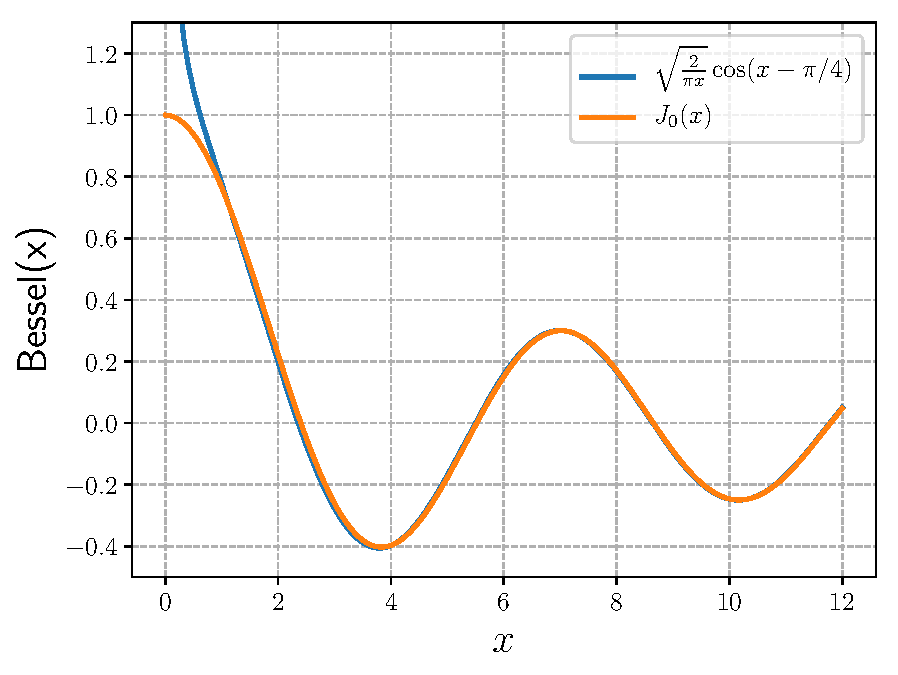
\includegraphics[width=0.75\textwidth]{./plots/pdf/strogatz-wk05-bessel.pdf}
	\caption{Plotting the exact Bessel integral defined by eqn. \ref{eqn:bessel-zero} and its asymptotic approximation given by eqn. \ref{eqn:bessel-approx}.}
	\label{fig:strogatz-wk05-bessel}
\end{figure}

\paragraph{Example 5:} Next consider the function
\begin{gather*}
	I(x) = \int_{0}^{1} t \me^{\mi x t^2} \md t \qquad x \rightarrow \infty
\end{gather*}
Here $\psi(t)=t^2$ has $\psi'=0$ at $t=0$. But $f(t)=t$ also vanishes there so we may not get the $O(x^{-1/2})$ scaling. This is a contrived example and can be done exactly. Indeed
\begin{align*}
	I(x) &= \frac{1}{2\mi x} \left(\me^{\mi x} - 1\right) \\
		&= O\left(\frac{1}{x}\right)
\end{align*} 
where we have made use of the substitution $\mi x t^2 = y$. 

\begin{itemize}
	\item What is the significance of Example 5?
\end{itemize}


\paragraph{Example 6:} Consider
\begin{gather}
	I(x) = \int_{0}^{\infty} \cos \left[x\left(\frac{t^3}{3}-t\right)\right] \md t \label{eqn:wk5-ex6}
\end{gather}
Begin by plotting the integrand (Fig. \ref{fig:strogatz-wk05}).
\begin{figure}[h]
	\centering
	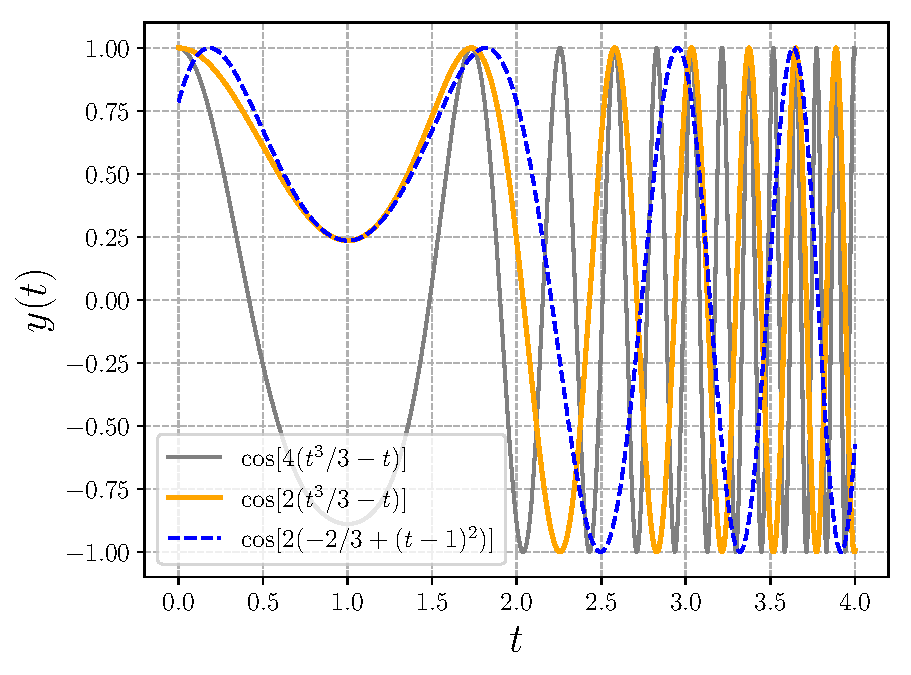
\includegraphics[width=0.75\textwidth]{./plots/pdf/strogatz-wk05-cos.pdf}
	\caption{Plotting the integrand of eqn. \ref{eqn:wk5-ex6} for two different values of $x$. As $x$ doubles, so does the frequency. The Taylor expansion about the stationary point $t=1$, eqn. \ref{eqn:psi-Taylor}, is also plotted.}
	\label{fig:strogatz-wk05}
\end{figure}\\
The phase is stationary when $t = \pm 1$. Since $0\leq t \leq \infty$, we only expand about the positive root. Taylor expanding
\begin{gather}\label{eqn:psi-Taylor}
	\psi(t) \approx -\frac{2}{3} + (t-1)^2
\end{gather}
This results in 
\begin{align*}
	I(x) &\sim \int_{0}^{\infty} \cos \left[-\frac{2x}{3} + x(t-1)^2\right] \md t \\
	& \sim \int_{-1}^{\infty}  \cos \left[-\frac{2x}{3} + xs^2\right] \md s
\end{align*}
We can extend the limit $-1$ to $-\infty$ as we expect it to not affect the leading order term (affects higher order terms). Also note that we Taylor expand only about one of the stationary points in writing the relation \ref{eqn:psi-Taylor}. So even as we extend the domain to include $t=-1$, it won't provide a dominant contribution. Then
\begin{align*}
	I(x) &\sim \int_{-\infty}^{\infty}  \cos \left[-\frac{2x}{3} + xs^2\right] \md s \\
	& \sim \cos \left(\frac{2x}{3}\right) \underbrace{\int_{-\infty}^{\infty}\cos (xs^2) \md s}_{\sqrt{\frac{\pi}{2x}}} + \sin \left(\frac{2x}{3}\right) \underbrace{\int_{-\infty}^{\infty}\sin (xs^2) \md s}_{\sqrt{\frac{\pi}{2x}}} \\
	& \sim \sqrt{\frac{\pi}{x}}\cos \left(\frac{2x}{3} - \frac{\pi}{4}\right)
\end{align*}
These Fresnel integrals are easily worked out using the complex Gaussian integral (eqn. \ref{eqn:complex-gauss-integral}) with $-\mi \rightarrow \mi$ and the scale transformation $\sqrt{x}s=t$. 


